\subsection{Literature Survey}
This chapter contains the literature analysis of the research papers that have been reviewed for the project. The papers have been categorized into two main sections: Landmark-Based Navigation Systems and Optimization and Fairness in Ride-Hailing Allocation Systems. The papers have been reviewed based on their relevance to the project and the insights they provide for the development of the proposed system. The literature review provides a comprehensive understanding of the existing research in the field and highlights the gaps that the proposed system aims to address.
\subsubsection{Related Work}
\subsubsection*{Landmark-Based Navigation Systems}

Landmark-based wayfinding plays a pivotal role in navigation. In a notable study, \textit{Rousell and Zipf} \cite{rousell-2017} primarily focus on the identification of appropriate landmarks for the generation of landmark-based navigation instructions by leveraging OpenStreetMap (OSM). This research identifies various prospective landmarks within a certain proximity to the user’s location (decision point) and in the intended direction toward the final destination. The study assigns attributes such as visual/semantic saliency, distance from the waypoint, visibility, position, location, and uniqueness to these landmarks. These attributes form a comparison basis for different landmarks, aiding in the selection of the most useful one through an iterative process. However, the approach is entirely reliant on OSM data and produces poor results in less explored geographic areas that have not been marked on OSM. Future work includes the selection of more popular landmarks by considering public perception and the investigation of more optimized techniques for the process.

A pioneering study by \textit{Anita Graser} \cite{graser-2017} paved the way for using OpenStreetMap as a prominent source for generating navigation instructions for pedestrians. A contemporary to \textit{Rousell and Zipf} \cite{rousell-2017}, this study introduced the concept of using landmarks for pedestrian navigation. An interesting proposal by the study was that landmarks were selected based on their relevance to the user's current location and the intended direction of travel. The approach was evaluated using a dataset of pedestrian routes in Vienna, Austria. However, the study was limited to a single city, and future research could explore the generalizability of the approach to other urban areas. As mentioned by \textit{Millonig et al.}, \textit{Graser's} study could be further improved upon consideration of "self-explaining" \cite{millonig-2021} environments, which would greatly benefit human wayfinding.

Another study by \textit{Löwen and Schwering} \cite{lowen-2020} presents an algorithm for the selection of route-dependent orientation information that emphasizes the significance of landmarks in human wayfinding and distinguishes itself from previous implementations by not only focusing on the selection of landmarks around the decision point but also along the route. The algorithm utilizes orientation information to better understand the spatial relationships between regions, thereby enhancing navigational effectiveness. However, it relies on the manual assignment of category weights for feature relevance, indicating a potential area for improvement. Further research could explore more sophisticated approaches for this process, possibly enhancing the algorithm's efficiency and adaptability.

Recently, algorithms to generate navigation instructions by representing them as Graph-to-Text problems has led in the development of deep-learning models and methodologies to generate such instructions in natural language. One such novel approach is taken by \textit{Schumann and Riezler} \cite{schumann-riezler-2021-generating} wherein they they evaluate rule-based as well as transformer based approaches for generation. The study focuses on generating instructions for pedestrian navigation by leveraging OpenStreetMap data.


The surge in application of Vision and Language Navigation (VLN) models has led to development of various other datasets, and tasks for evaluating, and improving efficiency of such models. \textit{Gu et al.} have categorized classes of solutions according to the challenges they solve \cite{gu-2022}. The importance of spatial understanding is well highlighted by the examples of 3D synthetic navigation environments such as \textit{LANI} \cite{misra-etal-2018-mapping}. The study also touched upon the importance of utilizing external knowledge, ie the interaction of objects with the AI agents, for making better navigation instructions. The study calls upon for the fact that using Google Street View images face potential problems on generalization for rest of the world, and hence, the need for more diverse dataset and user interaction is required.
To evaluate the performace of both models, they introduced the \textit{map2seq} dataset, which later became a benchmark for evaluating the performance of Vision and Language Navigation models \cite{schumann-riezler-2022-map2seq-vln} for instructions.
\textit{Staniek et al.} \cite{staniek-2024} offer another perspective on improving user\ interaction with landmark-based navigation systems by providing a powerful tool to simplify the task of OverpassQL query creation, enabling users to effortlessly query OSM using natural language without prior knowledge of OverpassQL. The approach explores and utilizes various evaluation metrics to compare the results of generating natural language queries by fine-tuning a sequence-to-sequence model on a self-created dataset, OverpassNL (which consists of natural language queries and corresponding OverpassQL queries), with large language models and few-shot examples. Although the latter approach showed better execution accuracy, it comes with its own computational cost and inefficiencies in misunderstanding and generating erroneous queries. The research leaves room for improvement in the semantic parsing of geographical data and the generation of more accurate OverpassQL queries from natural language.

\subsubsection*{Optimization and Fairness in Ride-Hailing Allocation Systems}
Allocation systems in ride-hailing services have been the focus of various research efforts aimed at optimizing rider-driver matching, improving fairness, and enhancing system efficiency.
\textit{Cui et al.} \cite{cui-2022} explore strategies for optimizing ride allocation, emphasizing customer satisfaction and minimizing delays. However, they highlight limitations posed by traffic conditions, which vary across dynamic environments. Future research is suggested to incorporate factors like weather conditions and autonomous systems to make the model more adaptive to urban environments.

Addressing the issue of fairness in ride-hailing platforms, \textit{Kang et al.} \cite{kang-2024} utilize the Markov Decision Process (MDP) to ensure equitable distribution of riders to drivers over time. Although the study achieves a balanced allocation, it struggles when confronted with real-world disruptions, which can lead to inefficient rider-driver matching. Future advancements in this area could focus on adapting fairness models to manage more complex and unpredictable real-world environments, ensuring both equity and system efficiency.

Proposing a dynamic programming approach, \textit{Singhal and Pandey} \cite{singhal-2016} solve the classical Travelling Salesman Problem, which has implications for ride allocation and its further optimization. Their approach involves optimizing routes and minimizing distances, thus reducing both route lengths and travel times efficiently. However, the algorithm performs poorly with multiple objectives, suggesting a need for future research to find better ways to address this issue, primarily focusing on adaptive algorithms in dynamic environments.

Focusing on fairness in rider allocation, \textit{Cao et al.} \cite{cao-2021} developed an algorithm that optimizes routes while ensuring that no user faces unnecessary delays, which is highly relevant for driver allocation systems. However, the algorithm struggles in large dynamic environments, where fair and efficient ride allocation becomes complex. Future work could focus on dynamic pricing models and extending the approach to handle fleets of shared electric vehicles, ultimately enhancing driver and ride allocation in increasingly congested urban areas.

\textit{Martins et al.} \cite{martins-2024} highlight the socioeconomic factors related to ride-hailing systems in developing countries. The paper discusses how ride-sourcing services have created new opportunities for drivers while also posing challenges related to regulation and urban congestion. These issues directly impact how rides are allocated to drivers, as inconsistent regulatory frameworks and varying urban infrastructures can lead to inefficiencies in driver deployment. The future of this study involves developing better-suited models for traffic-dense and populated urban environments.


{\fontsize{10}{12}\selectfont % Adjust text size here
\begin{longtable}{|c|p{1.75cm}|c|p{2cm}|p{2cm}|p{2cm}|p{2cm}|}
    \caption{Research Contributions by Team Members} \\
    \hline
    \textbf{S. No.} & \textbf{Roll Number} & \textbf{Name} & \textbf{Paper Title} & \textbf{Tools / Technology Used} & \textbf{Findings} & \textbf{Citation} \\ \hline
    \endfirsthead
    %
    \multicolumn{7}{c}{{\textbf{Table \thetable\ Continued from previous page}}} \\ \hline
    \textbf{S. No.} & \textbf{Roll Number} & \textbf{Name} & \textbf{Paper Title} & \textbf{Tools / Technology Used} & \textbf{Findings} & \textbf{Citation} \\ \hline
    \endhead
    %
    \hline
    \multicolumn{7}{|r|}{{\textbf{Continued on next page}}} \\ \hline
    \endfoot
    %
    \hline
    \endlastfoot
    %
    1 & 102116122 & Ansh Midha & Traffic-Aware Ride Allocation & Traffic Models, Dynamic Programming & Improved ride allocation using traffic data; struggled under extreme conditions. & Cui et al. \cite{cui-2022}  \\ \hline
    2 &           &           & Fairness in Rider-Driver Matching & Markov Decision Process (MDP) & Addressed fairness concerns; struggled with dynamic real-world changes. & Kang et al. \cite{kang-2024} \\ \hline
    3 &           &           & Route Optimization in Allocation Systems & Travelling Salesman Problem (TSP), Optimization Models & Optimized route allocation; multi-objective handling needs improvement. & Singhal and Pandey \cite{singhal-2016} \\ \hline
    4 & 102116115 & Leena Gupta & Landmark-Based Navigation Using OSM & OSM, OverpassQL & Landmark identification improves navigation; underperformance in poorly mapped areas. & Rousell and Zipf \cite{rousell-2017} \\ \hline
    5 &           &           & Pedestrian Navigation Using Landmarks & OSM, Spatial Algorithms & Highlighted relevance of landmarks; limited generalization outside urban environments. & Graser \cite{graser-2017} \\ \hline
    6 &           &           & Human-Centric Orientation for Wayfinding & Route Visualization, Spatial Algorithms & Enhanced orientation for navigation by emphasizing route landmarks. & Löwen and Schwering \cite{lowen-2020} \\ \hline
    7 & 102116082 & Madhur Gaba & Dynamic Pricing for Ride-Hailing Optimization & Pricing Algorithms, Traffic-Aware Systems & Optimized dynamic pricing models for better ride allocation. & Cui et al. \cite{cui-2022} \\ \hline
    8 &           &           & Real-Time Ride-Hailing Allocation & Traffic Models, Dynamic Environment Analysis & Proposed strategies for real-time ride optimization under variable conditions. & Singhal and Pandey \cite{singhal-2016} \\ \hline
    9 & 102116106 & Shourya De & Equitable Allocation for Ride-Hailing Systems & Fairness Algorithms, Congestion Analysis & Ensured fairness but struggled with efficiency under dynamic loads. & Cao et al. \cite{cao-2021} \\ \hline
    10 &          &           & Socioeconomic Analysis of Ride-Hailing Systems & Socioeconomic Data, Traffic Analysis & Analyzed inefficiencies in ride-hailing in developing countries. & Martins et al. \cite{martins-2024} \\ \hline
    11 &          &           & Graph-Based Instruction Generation for Navigation & Graph-to-Text Models, OSM Data & Improved textual navigation instruction generation using graphs. & Schumann et al. \cite{schumann-riezler-2021-generating} \\ \hline
    12 & 102166002 & Yash Dogra & Vision and Language Navigation Models & VLN Models, Transformer Networks, map2seq Dataset & Improved navigation using graph-to-text natural language instructions. & Schumann and Riezler \cite{schumann-riezler-2022-map2seq-vln} \\ \hline
    13 &          &           & 3D Synthetic Environments for Navigation & LANI Platform, Spatial Understanding Models & Provided controlled testing environments for spatial AI agents. & Gu et al. \cite{gu-2022}, LANI \cite{gu-2022} \\ \hline
    14 &          &           & OverpassQL Queries Using Natural Language & OverpassQL, Seq2Seq Models & Simplified querying of OSM; computationally expensive on large datasets. & Staniek et al. \cite{staniek-2024} \\ \hline
\end{longtable}
}


\subsubsection{Research Gaps of Existing Literature}

\begin{table}[H]
	\centering
	\caption{Mapping Research Objectives to Related Research Gaps}
	\fontsize{10}{12}\selectfont
	\label{tab:research-gaps}
	\begin{tabularx}{\textwidth}{|X|X|X|}
		\hline
		\textbf{Research Objective}              & \textbf{Related Research Gaps}                                                                      & \textbf{Relevant Studies}                                                            \\
		\hline
		\textbf{Better Navigation}               & Landmark identification relies heavily on OSM data, leading to poor results in less explored areas. & \textit{Rousell and Zipf} \cite{rousell-2017}, \textit{Graser} \cite{graser-2017}    \\
		\hline
		\textbf{Real-Time E-Rickshaw Monitoring} & Ride allocation systems struggle with real-time traffic conditions and dynamic environments.        & \textit{Cui et al.} \cite{cui-2022}, \textit{Singhal and Pandey} \cite{singhal-2016} \\
		\hline
		\textbf{Campus Specific Routing}         & Limited generalizability of routing in TIET, aptly tackling road blockage.                          & \textit{Kang et al.} \cite{kang-2024}, \textit{Cao et al.} \cite{cao-2021}           \\
		\hline
	\end{tabularx}
\end{table}



\subsubsection{Detailed Problem Analysis}

\subsubsection*{1. Navigating through the Unfamiliar Campus}
Newly admitted students and visitors frequently encounter challenges when attempting to navigate expansive, complicated, and unfamiliar campus environments. Traditional text-based navigation is not always intuitive, and visual maps can be overwhelming, especially when users need to follow a series of steps to arrive at their destination.

\textbf{Problem:}
\begin{itemize}
	\item \textbf{Lack of personalization:} Static maps cannot meet individual needs, such as identifying the most efficient route or recognizing landmarks that are easy to spot.
	\item \textbf{Elaborate navigation instructions:} Existing text-based navigation guidelines often require users to mentally visualize directions, which is prone to error.
	\item \textbf{Poor use of landmarks:} Landmarks can serve as intuitive reference points for users; however, current navigation systems do not always recognize or recommend relevant landmarks based on user context (location, preferences).
\end{itemize}

\textbf{Goal:} To design an innovative, user-friendly navigation system that helps users easily understand and follow campus routes using landmarks and visual aids.

\subsubsection*{2. Real-Time Monitoring of Electric Rickshaws}
Electric rickshaws are commonly used as a form of transport on campus; however, users often face difficulties in estimating wait times and vehicle availability, leading to frustration.

\textbf{Problem:}
\begin{itemize}
	\item \textbf{No real-time monitoring:} Users cannot receive updates on the location or availability of e-rickshaws, leading to unpredictability and poor planning.
	\item \textbf{Indeterminate arrival times:} Current systems cannot provide an accurate estimate of when a vehicle will reach a specific location, impacting users' ability to plan effectively.
	\item \textbf{Limited awareness of vehicle availability:} Without real-time data, students and visitors may end up waiting unnecessarily or miss available vehicles.
\end{itemize}

\textbf{Objective:} To implement a real-time e-rickshaw hailing platform with live updates on availability, location, and hailing services, enhancing overall efficiency and satisfaction.

\subsubsection*{3. Suggested Features for Iconic Campus Locations}
Campus users, including students, staff, and visitors, often need guidance to reach popular locations, such as cafeterias, academic buildings, or administrative offices.

\textbf{Problem:}
\begin{itemize}
	\item \textbf{Limited guidance for visitors:} Newcomers or visitors may not know where to find the most frequently visited sites and may rely on others for directions.
	\item \textbf{Static maps and directories:} Existing systems do not provide personalized recommendations or prioritize locations based on the user’s needs (e.g., a first-time student may not be interested in administrative offices but may need to know the closest cafeteria).
	\item \textbf{Lack of dynamic routing:} Existing solutions do not cater to real time updates on road blockages and other necessary detours.
\end{itemize}

\textbf{Objective:} To develop a recommendation system that highlights popular campus locations based on real-time data, user preferences, and situational factors, such as time of day, ongoing events, or personal inputs.


\subsubsection{Survey of Tools and Technologies used}
The related work reviewed for this study utilizes a diverse range of tools, technologies, and methodologies. Below is a categorized survey of these elements based on their usage and application:

\textbf{1. Landmark-Based Navigation Systems}
\begin{itemize}
	\item \textbf{OpenStreetMap (OSM):} A widely used, open-source geographic information system (GIS) employed by \textit{Rousell and Zipf} \cite{rousell-2017} and \textit{Graser} \cite{graser-2017} for extracting landmark data and generating navigation instructions.
	\item \textbf{OverpassQL:} Used by \textit{Staniek et al.} \cite{staniek-2024} to query OSM for specific landmarks and geospatial data. Fine tuned seq-2-seq models were also trained to generate OverpassQL queries from natural language.
	\item \textbf{Vision and Language Navigation (VLN) Models:} Deep learning-based models such as transformer architectures, as discussed by \textit{Schumann and Riezler} \cite{schumann-riezler-2021-generating}, for generating natural language navigation instructions.
	\item \textbf{map2seq Dataset:} Introduced by \textit{Schumann et al.} \cite{schumann-riezler-2022-map2seq-vln} for training and evaluating VLN models on tasks requiring spatial reasoning and textual instruction generation.
	\item \textbf{Synthetic Navigation Environments:} Platforms like \textit{LANI} \cite{misra-etal-2018-mapping}, which provide controlled 3D virtual environments to train and evaluate navigation models.
\end{itemize}

\textbf{2. Optimization and Fairness in Ride-Hailing Allocation Systems}
\begin{itemize}
	\item \textbf{Markov Decision Process (MDP):} Utilized by \textit{Kang et al.} \cite{kang-2024} to ensure equitable rider-driver matching over time.
	\item \textbf{Dynamic Programming:} Applied by \textit{Singhal and Pandey} \cite{singhal-2016} to solve the Travelling Salesman Problem, which has direct implications for optimizing ride allocation.
	\item \textbf{Socioeconomic Data Analysis:} \textit{Martins et al.} \cite{martins-2024} leveraged socioeconomic data and urban traffic models to explore challenges specific to ride-hailing systems in developing countries.
	\item \textbf{Traffic-Aware Algorithms:} \textit{Cui et al.} \cite{cui-2022} incorporated traffic condition data to improve allocation systems but noted gaps in handling weather and environmental changes.
	\item \textbf{Fairness-Oriented Algorithms:} Algorithms developed by \textit{Cao et al.} \cite{cao-2021} to minimize delays and optimize fairness in ride allocation while considering urban congestion dynamics.
\end{itemize}

\textbf{3. Common Tools and Datasets Across Related Work}
\begin{itemize}
	\item \textbf{Geospatial APIs and Frameworks:} APIs like OSM and tools such as Overpass API play a critical role in navigation and allocation research.
	\item \textbf{Machine Learning Models:} Transformer-based models and sequence-to-sequence architectures are commonly employed in language-to-query or navigation instruction tasks.
	\item \textbf{Evaluation Metrics:} Research often uses task-specific benchmarks such as map2seq dataset performance and natural language query accuracy to evaluate system effectiveness.
\end{itemize}

This survey highlights the wide range of technologies that have advanced navigation and ride allocation systems, while also identifying gaps and challenges that need to be addressed in future research.


\subsubsection{Summary}

The existing body of work on landmark-based navigation systems and ride-hailing allocation systems provides a solid foundation for addressing the challenges of campus navigation and e-rickshaw allocation. Landmark-based navigation systems, such as those proposed by \textit{Rousell and Zipf} \cite{rousell-2017} and \textit{Graser} \cite{graser-2017}, focus on using OpenStreetMap (OSM) data to generate navigation instructions, but these approaches often fall short in less-mapped regions or fail to incorporate user-generated insights. Similarly, advanced algorithms for ride-hailing, such as those developed by \textit{Cui et al.} \cite{cui-2022} and \textit{Kang et al.} \cite{kang-2024}, optimize allocation but are often limited by dynamic real-world disruptions or computational overheads.

This work builds on these studies by integrating key concepts such as:
\begin{itemize}
	\item Leveraging OSM data for navigation while addressing gaps in underrepresented areas by incorporating real-time user inputs and preferences.
	\item Combining pedestrian navigation and ride-hailing systems into a unified campus-specific solution, tailored to the unique needs of students and visitors.
	\item Enhancing ride allocation efficiency by focusing on campus-specific environmental factors, such as e-rickshaw availability, routes, and closures.
	\item Introducing a recommendation feature to highlight popular campus landmarks and facilities based on user feedback, a novel approach not explored in the reviewed literature.
\end{itemize}

While previous studies have explored navigation and allocation systems independently, this work aims to merge these domains into a single, context-aware application specifically designed for the TIET campus environment. By addressing the limitations of reliance on static data, underdeveloped regions, and isolated system functionalities, this research contributes to creating a more dynamic and inclusive solution for campus navigation and e-rickshaw management.

\subsection{Software Requirement Specification}

The following section details the software requirements necessary for the development and implementation of MapMitra.

\subsubsection{Introduction}

The following outlines the foundational aspects of the software requirements for MapMitra:

\subsubsection*{Purpose}
MapMitra aims to enhance campus navigation and transportation efficiency by integrating landmark-based directions with real-time e-rickshaw tracking. The objective is to provide an intuitive and user-friendly navigation experience for new students, visitors, and e-rickshaw users. This specification details the software requirements necessary for developing a robust application that meets the diverse needs of its users.

\subsubsection*{Intended Audience and Reading Suggestions}
The usage of this document is intended for stakeholders involved in the development and deployment of the campus navigation system, including PMSs, software developers, UI/UX designers, and QA teams. Additionally, it serves as a reference for end-users, administrators, and any parties responsible for system maintenance. Readers are encouraged to review the requirements to understand the application's capabilities, constraints, and design considerations.

\subsubsection*{Project Scope}
MapMitra focuses on creating a comprehensive navigation system tailored to the college campus. The system includes a digital map with landmark-based directions and real-time tracking for e-rickshaws, aimed at improving navigation and transportation efficiency. The scope covers the design, implementation, testing, and deployment of the application, emphasizing user-friendliness and efficiency. The project relies on existing campus maps and GPS data and does not involve hardware components.

\subsubsection{Overall Description}

\subsubsection*{Product Perspective}
MapMitra is an innovative solution for campus navigation and transportation. By integrating digital mapping with real-time e-rickshaw tracking, the application offers an interactive and intuitive user experience. Utilizing modern web technologies, the application is compatible with various devices and platforms. MapMitra features easy navigation through familiar landmarks and efficient e-rickshaw management, making it a valuable tool for the campus community.

\subsubsection*{Product Features}
MapMitra has the following features:
\begin{itemize}
	\item \textbf{Landmark-Based Navigation:} Provides directions using well-known campus landmarks and natural language instructions, simplifying navigation for new students and visitors.
	\item \textbf{Real-Time E-Rickshaw Tracking:} Displays live locations and estimated arrival times for nearby e-rickshaws, improving efficiency and reducing wait times.
	\item \textbf{Auto Driver Interface:} Provides e-rickshaw drivers with a platform to view and manage ride requests, ensuring smooth handling of transportation needs.
	\item \textbf{Admin Flow Management:} Allows administrators to add new routes, register auto drivers, and manage road closures, keeping the system accurate and relevant.
\end{itemize}

\noindent Figure \ref{fig:gmaps} shows what new features the various target groups want a common routing software, in this case Google Maps, to include.

\begin{figure}[H]
	\centering
	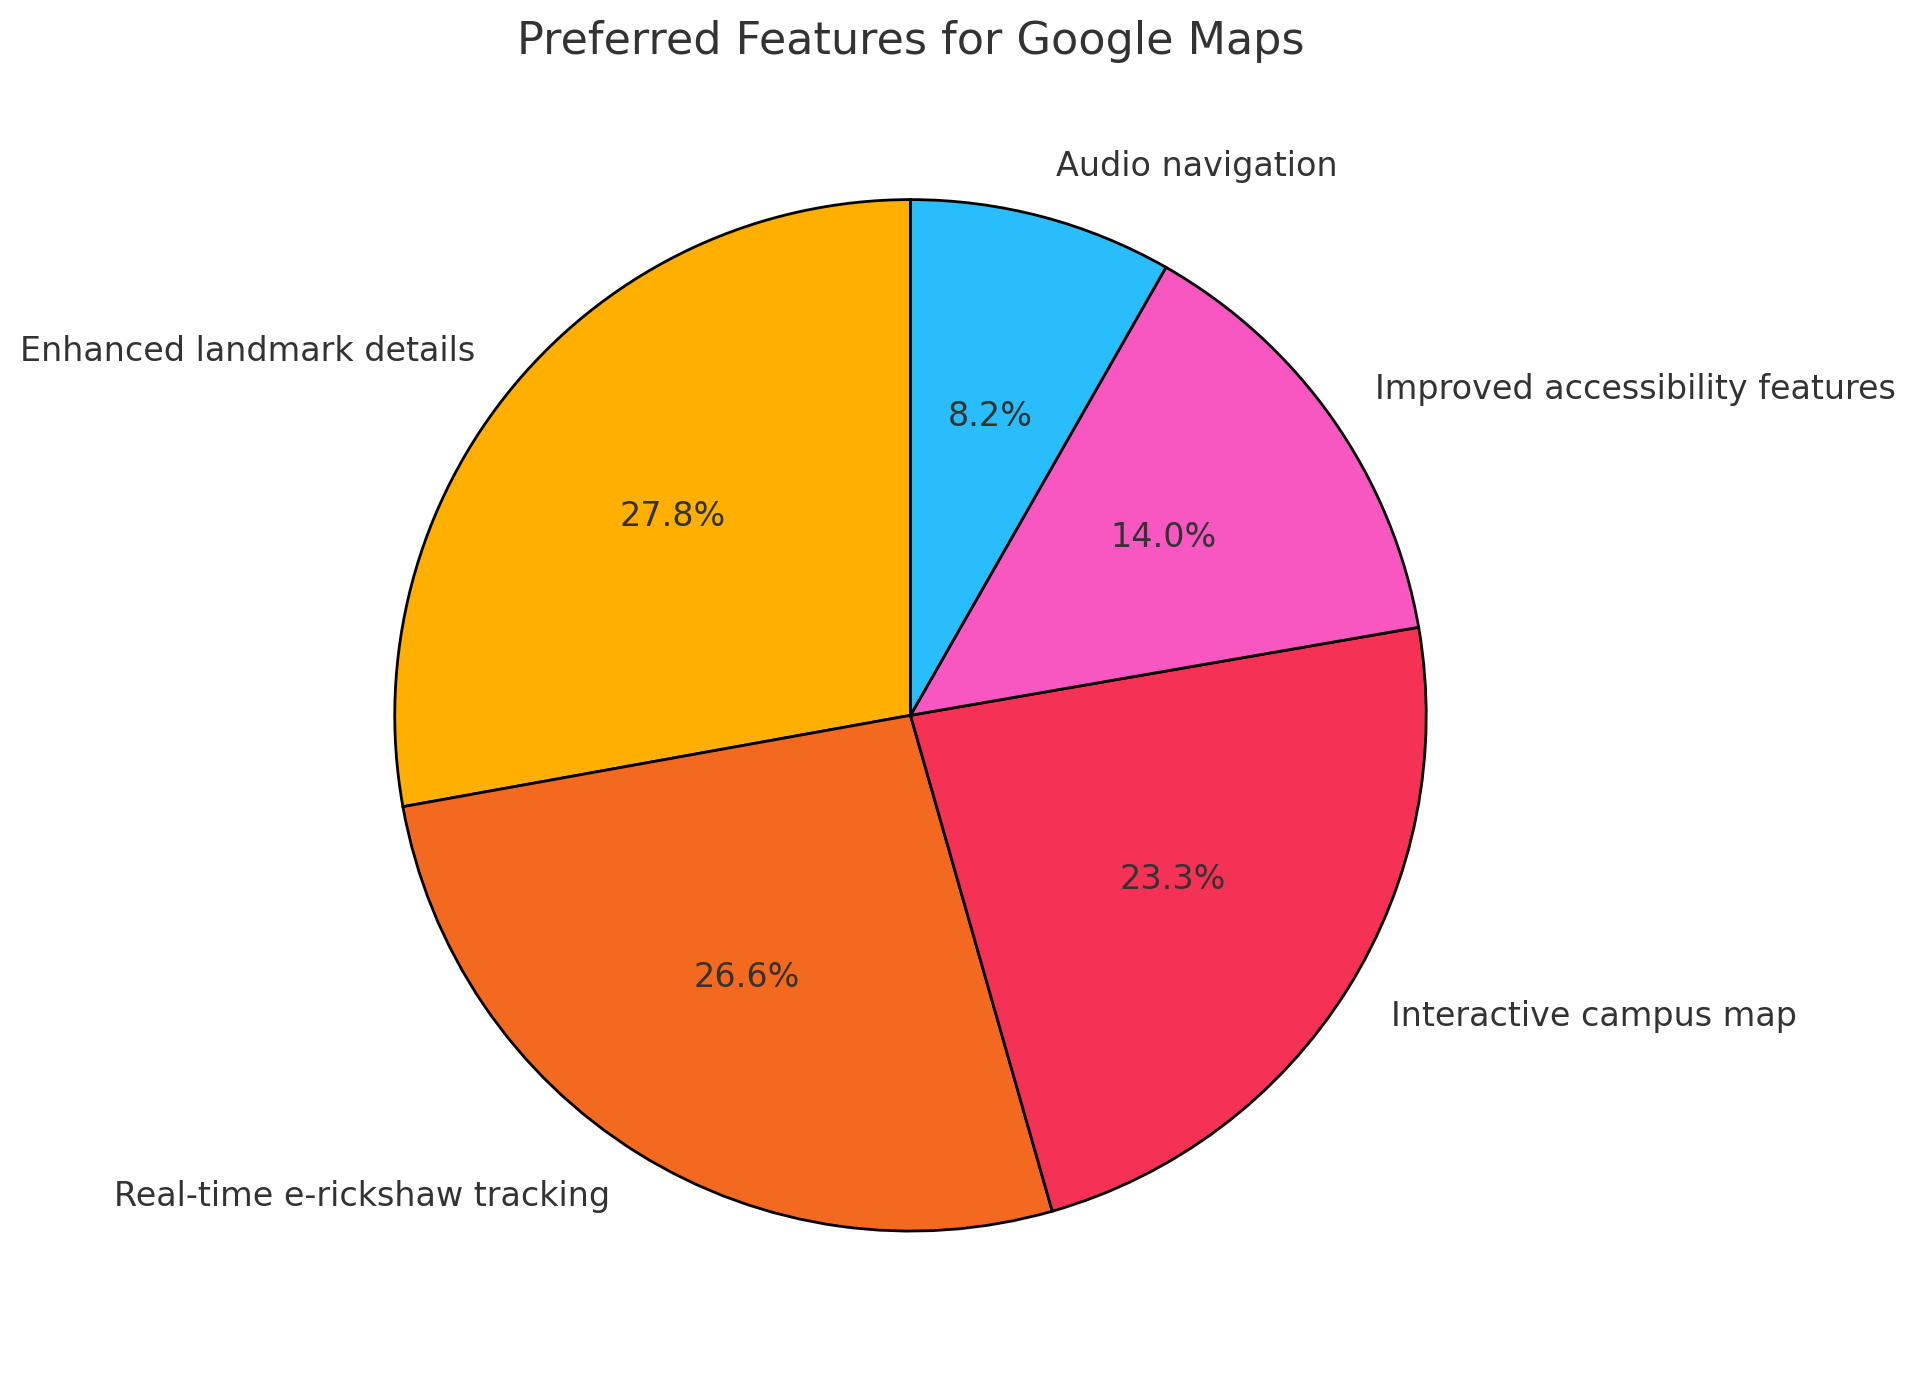
\includegraphics[width=0.75\textwidth]{vis3.png}
	\caption{Preferred features for google maps}
	\label{fig:gmaps}
\end{figure}

\subsubsection{External Interface Requirements}

\subsubsection*{User Interfaces}
MapMitra's user interface is designed to be intuitive and engaging, featuring:
\begin{itemize}
	\item An interactive campus map with real-time navigation elements.
	\item Updates on e-rickshaw availability and estimated arrival times.
	\item A recommendation engine with filters and detailed information on suggested amenities.
	\item An interface for auto drivers to manage ride requests and availability.
\end{itemize}

\subsubsection*{Hardware Interfaces}
Though the project does not involve specific hardware, it relies on:
\begin{itemize}
	\item GPS tracking in e-rickshaws for real-time tracking.
	\item Standard mobile and web browsers for accessing the application.
\end{itemize}

\subsubsection*{Software Interfaces}
MapMitra integrates with:
\begin{itemize}
	\item \textbf{Campus Map Data:} Digital campus maps for accurate navigation.
	\item \textbf{GPS Tracking Systems:} GPS data from e-rickshaws to provide real-time location updates.
	\item \textbf{External Services:} APIs for user authentication, map services, and recommendation systems.
\end{itemize}

\subsubsection{Other Non-Functional Requirements}

\subsubsection*{Performance Requirements}
\begin{itemize}
	\item \textbf{Speed and Responsiveness:} Ensure quick and responsive navigation and request handling, minimizing latency.
	\item \textbf{Concurrency Handling:} Efficiently manage multiple concurrent requests without performance degradation.
\end{itemize}

\subsubsection*{Safety Requirements}
\begin{itemize}
	\item \textbf{Data Privacy:} Implement strong encryption and authentication measures to protect user data and comply with privacy regulations.
	\item \textbf{Error Handling:} Provide comprehensive error handling to manage unexpected issues and offer users clear messages and recovery options.
\end{itemize}

\subsubsection*{Security Requirements}
\begin{itemize}
	\item \textbf{Access Control:} Secure user authentication and authorization to prevent unauthorized access to sensitive information.
	\item \textbf{Data Protection:} Safeguard user data through secure storage and transmission practices.
	\item \textbf{Regular Audits:} Conduct regular audits and system assessments to ensure integrity and security.
\end{itemize}

\subsection{Cost Analysis}
In the context of MapMitra, a direct financial cost analysis is not applicable as the project does not involve significant hardware investments or physical resources.

\subsection{Risk Analysis}

\subsubsection*{Software Risks}
\begin{itemize}
	\item \textbf{Integration Challenges:} Potential difficulties may arise when merging real-time GPS data with the navigation system, which could lead to functionality issues.
	\item \textbf{Performance Issues:} High user loads or unoptimized code may result in slow response times or crashes, impacting overall system performance.
	\item \textbf{Software Bugs:} Undetected bugs or errors could lead to unpredictable behavior, affecting the user experience and system stability.
\end{itemize}
\textbf{Impact:} These risks could significantly impact system performance. However, the likelihood of such issues occurring is considered low.

\subsubsection*{Technical Risks}
\begin{itemize}
	\item \textbf{Map Data Accuracy:} Outdated or incorrect map data could result in erroneous navigation instructions, compromising user experience.
	\item \textbf{GPS Tracking Reliability:} Issues with GPS tracking could impact real-time updates of e-rickshaw locations, leading to inaccurate information for users.
	\item \textbf{System Compatibility:} Compatibility challenges with various devices or operating systems might impact the application's performance across different platforms.
	\item \textbf{Security Vulnerabilities:} Weaknesses in the software could pose security risks, potentially leading to breaches or misuse of data.
\end{itemize}
\textbf{Impact:} These risks could significantly impact system performance. However, the likelihood of such issues occurring is considered low.
